\chapter{Emotion Classification Approaches}

In this chapter we will go through the experiments we made for this
project. Specifically, we will show how we tried to build some first models, solely 
based on the MoodyLyrics dataset, with no particular preprocessing nor feature
engineering techniques, just by using the tools we already mentioned. Then we will
move to more complex feature engineering techniques and classifiers.

Along with that, we will also provide a formal validation of the POS tagger tool we used.

%%%%%%%%%%%%%%%%%%%%%%%%%%%%%%%%%%%%%%%%%%%%%%%%%
%%%%%%%%%%%%%%%%%%%%%%%%%%%%%%%%%%%%%%%%%%%%%%%%%
%%%%%%%%%%%%%%%%%%%%%%%%%%%%%%%%%%%%%%%%%%%%%%%%%
%%%%%%%%%%%%%%%%%%%%%%%%%%%%%%%%%%%%%%%%%%%%%%%%%
%%%%%%%%%%%%%%%%%%%%%%%%%%%%%%%%%%%%%%%%%%%%%%%%%
\section{Public datasets}
A big challenge in emotion detection is the lack of a labelled emotion database to enable active innovation. Currently, few publicly accessible databases are available.\\\textit{MoodyLyrics}\cite{moodylyrics} contains around 2500 songs manually annotated through Amazon Mechanical Turk with 4 different emotion labels, i.e., happy, sad, angry and relaxed.\\
\textit{EmoInt}\cite{emoint} contains manually annotated tweets classified according to the intensities of anger, fear, joy and sadness. \textit{EmoBank}\cite{emobank} instead contains 10.000 sentences, each of which has been annotated according to both the emotion expressed by the writer and the emotion perceived by the reader.

Certainly, the most appropriate dataset for our problem among those we found is MoodyLyrics.

\subsection{MoodyLyrics}

As already mentioned, MoodyLyrics is a manually annotated dataset of 2595 songs labeled according to 4
different emotion labels: happy, sad, angry and relaxed.

MoodyLyrics creators used content words of lyrics and their valence and arousal norms to assign songs with those labels.
In particular, they used Russell's Valence-Arousal model with the 4 mood categories described for the annotation process\cite{russell1980circumplex}. Valence, which describes the pleasant-unpleasant degree, and Arousal, which describes aroused-sleepy degree, values of songs are computed adding the corresponding values of each word of lyrics that is found in a lexicon which was build by combining ANEW (Affect Norm of English Words), WordNet and WordNet-Affect. 

In the context of MoodyLyrics, Valence represents the positive or negative intensity of an emotion whereas Arousal indicates how strongly or rhythmically the emotion is felt\cite{moodylyrics}.

Based on this assumptions, MoodyLyrics creators classified lyrics according to the planar model shown in figure \ref{fig:ml-classification-schema}, which relates arousal and valence.

\begin{figure}[H]
  \centering
  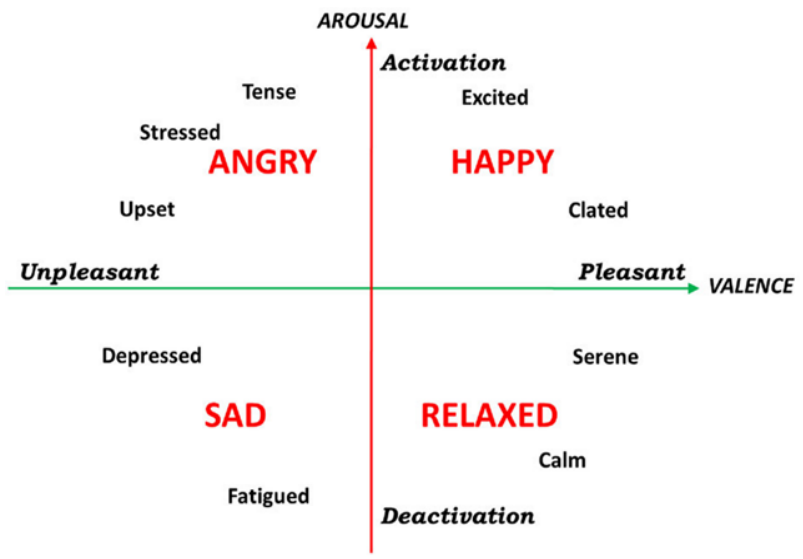
\includegraphics[width=0.6\textwidth]{./chapters/chapter4/images/moodylyrics-classification-schema}
  \caption{Valence and Arousal planar model used by MoodyLyrics creators to annotate lyrics\cite{moodylyrics}}
  \label{fig:ml-classification-schema}
\end{figure}

\subsubsection{MoodyLyrics duplicates bug}

During the analysis of MoodyLyrics described in the previous section we detected the presence of duplicated songs inside the dataset. Moreover, sometimes different emotions were associated with the duplicated songs. Thus, to continue our analysis we eliminated duplicated rows and we chose as emotion label the most frequent emotion between all the duplicates.\par

This bug in the dataset was reported to MoodyLyrics creators. As a response to our bug report email, MoodyLyrics creators suggested to use MoodyLyrics4Q\cite{moodylyrics4q}, that, according to them is a more accuratelly labeled version of MoodyLyrics.\par

This advice opened us three possibilities: continue using MoodyLyrics, start using MoodyLyrics4Q or create a new dataset as the concatenation of the previous two. We decided to start using all these three models, in order to understand which one, at the end, will give us a better playlists classification. The complete MoodyLyrics emotion classification analysis can be found at \href{https://github.com/sgiammy/emotion-patterns-in-music-playlists/blob/master/Notebook/1_ED_in_songs_lyrics.ipynb}{Notebook 1}, while the MoodyLyrics4Q and the emotion detection analysis in the merged datasets can be found at \href{https://github.com/sgiammy/emotion-patterns-in-music-playlists/blob/master/Notebook/2_Advanced_Feature_Engineering.ipynb}{Notebook 2}.


\subsection{MoodyLyrics4Q}
MoodyLyrics4Q contains 2000 songs and has the same annotation schema as MoodyLyrics. Figure \ref{fig:stats} shows the emotions distribution comparison between the two MoodyLyrics versions.

\begin{figure}[H]
\centering
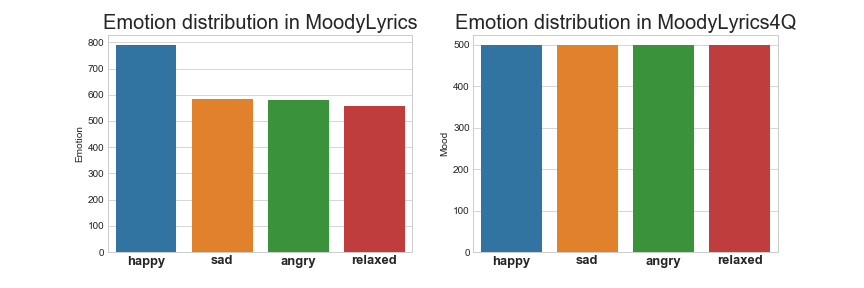
\includegraphics[width=1.1\textwidth]{./chapters/chapter4/images/Stats.png}
\caption{Emotions distribution comparison between MoodyLyrics and MoodyLyrics4Q}
\label{fig:stats}
\end{figure}

MoodyLyrics4Q classes are much more balanced, however MoodyLyrics4Q contains less songs with respect to MoodyLyrics. \par
We studied the qualitative difference between the two version comparing the classification given to the songs contained in both datasets to establish what version, according to us, is more correct. The intersection between the two versions contains 47 songs, and 21 over 47 have been classified differently. We noticed that in 15 over this 21 songs the two datasets confuses \textit{happy} with \textit{relaxed} and \textit{angry} with \textit{sad}. Indeed, only 6 of 21 songs are classified totally differently if we assume that we can merge happy and relaxed and angry and sad emotion. However, reading the lyrics of each of this 6 songs, we could not establish which version is the best one. A more detailed analysis can be fount at \href{https://github.com/sgiammy/emotion-patterns-in-music-playlists/blob/master/Notebook/5_Final_steps.ipynb}{Notebook 5}. 

%%%%%%%%%%%%%%%%%%%%%%%%%%%%%%%%%%%%%%%%%%%%%%%%%
%%%%%%%%%%%%%%%%%%%%%%%%%%%%%%%%%%%%%%%%%%%%%%%%%
%%%%%%%%%%%%%%%%%%%%%%%%%%%%%%%%%%%%%%%%%%%%%%%%%
%%%%%%%%%%%%%%%%%%%%%%%%%%%%%%%%%%%%%%%%%%%%%%%%%
%%%%%%%%%%%%%%%%%%%%%%%%%%%%%%%%%%%%%%%%%%%%%%%%%
\section{POS Tagger Validity Check} 

Before digging into more complex types of analysis, we took the time to check if
the tools we were using could be really good for our purpose. \par

Specifically, we had some doubts on the Part-Of-Speech (POS) tagger. Indeed, those kind of systems are generarly 
trained on texts coming from sources whose type of language is very different from those
we would expect to find in lyrics. In fact, the SpaCy's POS tagger implemented in the language
model we are using is trained on OntoNotes 5\cite{ontonotes5} and on Common Crawl\cite{common-crawl},
which are both made of pieces of text taken from news, conversational telephone speech, weblogs, 
usenet newsgroups, broadcast and talk shows. Obviously, this type of natural language texts are 
much different from a lyric and we just wanted to make sure that we were using an appropriate tool.

Before going into the details of what we did, we must state that SpaCy's POS tagger provides two tags per words, which
will both be considered in our analysis. Those two types of tag are:

\begin{itemize}
\item \textbf{POS}: coarse-grained part-of-speech e.g. VERB
\item \textbf{TAG}: fine-grained part-of-speech e.g. PAST\_TENSE
\end{itemize}

In order to obtain reliable insights of the functionalities of our POS tagger we considered three songs:
one with a common language and very few slang words, one filled with slangs and another one with some
vulgar words.

The first song we considered was ``Polly'' from Nirvana.

As a first approach we tried to tag the words considering one line of the lyric at the time. Here is an example of
what we obtained:

\begin{lstlisting}
Polly wants a cracker
PROPN VERB DET NOUN 

Polly = PROPN NNP -> noun, proper singular
wants = VERB VBZ -> verb, 3rd person singular present
a = DET DT -> determiner
cracker = NOUN NN -> noun, singular or mass
\end{lstlisting}

As a first attempt, our POS tagger completelly succedeed in recognizing the phrase in the 
exact way we were expecting. In fact, the absence of weird words, e.g. slangs, made the
task much easier.

Because of the almost complete absence of punctuation marks in our lyrics, we expected
the POS tagger to fail while analyzing an entire song as whole. Instead, we were quite
surprised to see that SpaCy's POS tagger does one desirable thing for our goal:
it treats each line as a standalone sentence, even though they are not specifically separed by
a stopping mark. Therefore, the same positive behaviour we observed on the first line
was totally replicated on the other lines, giving us the exact tagging we were
expecting by visually inspecting our song's lyrics.

We omitted the entire tagging process output for brevity reasons.

Our first experiment served to the purpose of arriving to a conclusion: SpaCy's POS tagger
is a good tool for lyrics. However it did not solve our doubts about its ability of recognizing
"weirder" words such as slang words or abbreviations. For this reason, we moved on 
analysing the lyrics of ``Kiss You Back'', from Underground Kiss.

The first interesting thing we noticed was that the POS tagger properly recognized abbreviations such as "'ll".
Moreover, another important feature we noticed was clearly visible while tagging this line: ``Yeah, we chocolate cross-over''.
Indeed, here the word "chocolate" is used as a verb (even though chocolate is clearly not defined as a verb in 
the dictionary) and the POS tagger was able to recognize this exception. 
This is quite important because, in songs, those situations happen very often.

Other additional things we noticed while analyzing this song came our of the tagging output of the following line:

\begin{lstlisting}
Jus't havin' fun with it, man, know what I'm sayin'?
NOUN VERB NOUN ADP PRON PUNCT INTJ PUNCT VERB NOUN PRON VERB VERB PUNCT PUNCT 

Jus't = NOUN NNS -> noun, plural
havin' = VERB VBG -> verb, gerund or present participle
fun = NOUN NN -> noun, singular or mass
with = ADP IN -> conjunction, subordinating or preposition
it = PRON PRP -> pronoun, personal
, = PUNCT , -> punctuation mark, comma
man = INTJ UH -> interjection
, = PUNCT , -> punctuation mark, comma
know = VERB VB -> verb, base form
what = NOUN WP -> wh-pronoun, personal
I = PRON PRP -> pronoun, personal
'm = VERB VBP -> verb, non-3rd person singular present
sayin = VERB VBG -> verb, gerund or present participle
' = PUNCT '' -> closing quotation mark
? = PUNCT . -> punctuation mark, sentence closer
\end{lstlisting}

One very interesting result we can notice comes from the following two lines:
\begin{lstlisting}
havin' = VERB VBG -> verb, gerund or present participle and
ayin = VERB VBG -> verb, gerund or present participle
\end{lstlisting}

In fact it looks like our POS tagger is able to recognize verbs in their correct tense
even if they are abbreviated in an unconventional way.

One thing which really impressed us, was the word "man" being recognized to be an interjection from time to time. 
"An interjection is a part of speech that shows the emotion or feeling of the author. These words or phrases can 
stand alone or be placed before or after a sentence. Many times an interjection is followed 
by a punctuation mark, often an exclamation point"\footnote{\url{http://examples.yourdictionary.com/examples-of-interjections.html}}. 
This description perfectly fits with the usage of the word "man" in their contextes when it was recognized to be an interjection. 

Those kind of things are not trivial to detect and this ability of our POS tagger convinced us even more
of its impressive skills.

The last thing we were left to analyze at this point was a vulgar song. For this purpose we considered 
"The Ballad Of Chasey Lain", from Bloodhound Gang. 

In this case we have no special remarks to report. We can just say that everything was tagged and
recognized in the exact way we expected.

We did not report entire lyrics nor the full POS tagger output in the interest of brevity. However, those analysis are available on the public GitHub repository for this project, at \href{https://github.com/sgiammy/emotion-patterns-in-music-playlists/blob/master/Notebook/3_POS_tagger_verification.ipynb}{Notebook 3}.

%%%%%%%%%%%%%%%%%%%%%%%%%%%%%%%%%%%%%%%%%%%%%%%%%
%%%%%%%%%%%%%%%%%%%%%%%%%%%%%%%%%%%%%%%%%%%%%%%%%
%%%%%%%%%%%%%%%%%%%%%%%%%%%%%%%%%%%%%%%%%%%%%%%%%
%%%%%%%%%%%%%%%%%%%%%%%%%%%%%%%%%%%%%%%%%%%%%%%%%
%%%%%%%%%%%%%%%%%%%%%%%%%%%%%%%%%%%%%%%%%%%%%%%%%
\section{Initial Classification}

The first approaches to classify emotions we tried, were entirely based on converting
MoodyLyrics entries into features. Specifically, since MoodyLyrics simply provides the
artist and the title of its songs, we firstly downloaded the lyrics and then we built
word embedding vectors for them by using SpaCy's built-in methods, based on GloVe.
Those vectors we worked on are made of 300 dimensions.

MoodyLyrics songs were annotated according to the arousal and valence dimension of their lyric,
as explained above. Therefore we thought that, if we could be able to project the resulting
word embedding vector of each lyric in a bi-dimensional space, we could have been able to 
clearly see how they are separated.

In order to visualize the mentioned idea, we applied Principal Component Analysis (PCA) on
MoodyLyrics songs and plotted the resulting points in 2-dimensional space, as can be seen in figure \ref{fig:ml-pca}. However the resulting figure is not exactly what we were expecting.

\begin{figure}[H]
  \centering
  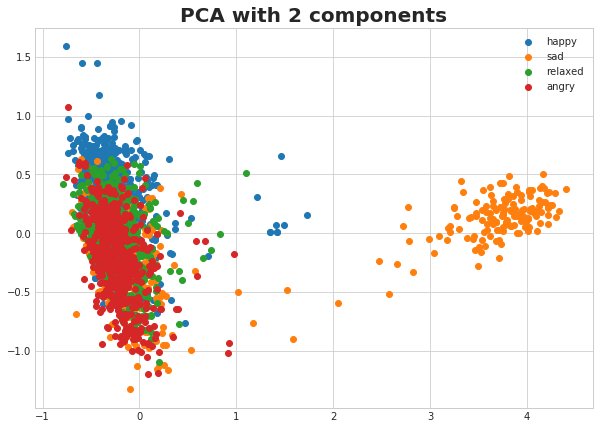
\includegraphics[width=0.7\textwidth]{./chapters/chapter4/images/ml-pca.png}
  \caption{Principal Component Analys on MoodyLyrics data with 2 dimensions as output}
  \label{fig:ml-pca}
\end{figure}

Indeed, because of the explained MoodyLyrics annotation schema, we were expecting to see 4 clearly separated group of points. Instead, what we can see is that sad songs are clearly separated from the others while the songs belonging to the classes happy, angry and relaxedare quite overlapped and can be easily confused between them.

Despite the fact that this result seemed weird, after listening to several songs and trying to
manually classify them according to their lyrics, we came to the conclusion that it is very
easy for a human to confuse happy, angry and relaxed song. Therefore, if we keep in mind that
MoodyLyrics was manually annotated, we can explain the anomaly in our plot as a consequence of human error during the annotation process.


After this preliminary data analysis, we moved on producing models to actually classify our dataset.
The result of these process are visible in table \ref{table:ml-simple-results} where the reported accuracy values were obtain after a 10-fold cross validation.
\begin{table}[H]
\centering
\begin{tabular}{@{}lll@{}}
\toprule
\textbf{Classifier} & \textbf{Accuracy})   \\ \midrule
k-Nearest Neighbour & 82\%  \\
Support Vector Machine & 90\%  \\
Gradient Boost & 86\%  \\
Neural Network & 90.55\%  \\
\end{tabular}
\caption{Accuracy results for different classifiers on MoodyLyrics}
\label{table:ml-simple-results}
\end{table}

As we can see, the best results were certainly achieved by a Neural Network whose architecture was as follows: one input layer with 175 neurons and sigmoid activation function, one hidden layer with 175 neurons and sigmoid activation function, one output layer with 4 neurons and softmax activation function.

Anyway for certain songs we noticed that the expressed emotion could be easily guessed from its title. Therefore
we tried to build also songs titles word embedding vectors and classified them. The results of this operation are 
visible in table \ref{table:ml-simple-results-title}. Again, those results were obtained after a 10-fold cross-validation. 

\begin{table}[H]
\centering
\begin{tabular}{@{}lll@{}}
\toprule
\textbf{Classifier} & \textbf{Accuracy})   \\ \midrule
Support Vector Machine & 67\%  \\
Gradient Boost & 65\%  \\
Neural Network & 70\%  \\
\end{tabular}
\caption{Accuracy results for different classifiers on MoodyLyrics, using just the title's word embedding vector}
\label{table:ml-simple-results-title}
\end{table}

Moreover, performances obtained while building classifiers based on the songs title's word embedding vector only
did not improve with respect to the previous case. Therefore we decided
that, probably, we could have given a try at using both the title's and the lyric's word embedding information for each
song. What we did was to use both lyrics vectors and title vectors norm. The results of this process are shown in table \ref{table:ml-simple-results-both}.

\begin{table}[H]
\centering
\begin{tabular}{@{}lll@{}}
\toprule
\textbf{Classifier} & \textbf{Accuracy})   \\ \midrule
Support Vector Machine & 91\%  \\
Neural Network & 54.14\%  \\
\end{tabular}
\caption{Accuracy results for different classifiers on MoodyLyrics, using both the lyric's and the title's word embedding vectors}
\label{table:ml-simple-results-both}
\end{table}


For this case we did not try to learn the same number of classifiers as above because, based on the previous experiments, we noticed
that SVM and ANN should be the best algorithms for our problem. 

The accuracy values obtained in this experiment seem quite abnormal. Indeed,
while the SVM provides an accuracy score which is comparable to those obtained while using only the lyrics content, the ANN performances 
drastically decreased. However, we were expecting to obtain performances very similar to those we got while using just the lyrics content as, 
in  this case, we are basically adding one features (which is the norm of the title's word embedding vector).

In conclusion, the best and more stable performances were those obtained by learning our model solely on the lyrics word embedding vectors.
Those results are also quite encouraging and made us think that, with some more advanced feature engineering techniques,
we may be able to achieve even better results.

%%%%%%%%%%%%%%%%%%%%%%%%%%%%%%%%%%%%%%%%%%%%%%%%%
%%%%%%%%%%%%%%%%%%%%%%%%%%%%%%%%%%%%%%%%%%%%%%%%%
%%%%%%%%%%%%%%%%%%%%%%%%%%%%%%%%%%%%%%%%%%%%%%%%%
%%%%%%%%%%%%%%%%%%%%%%%%%%%%%%%%%%%%%%%%%%%%%%%%%
%%%%%%%%%%%%%%%%%%%%%%%%%%%%%%%%%%%%%%%%%%%%%%%%%
\section{Feature Engineering}
In order to improve our model performances, we focused our attention on feature engineering. Specifically we tried to extract stylometric, structural, orientation and vocabulary based features\cite{features}. Apart from this we also generated a word embedding vector of the words contained in each song's lyric by using SpaCy's\cite{spacy} pre-trained language model based on GloVe\cite{glove}.\par

Here is a comprehensive list of the features we extracted from our dataset, followed by a brief description:

\begin{description}
\item \textbf{Title\_vector}: word embedding vector of the song's title
\item \textbf{Lyric\_vector}: word embedding vector of the lyric content
\item \textbf{\%Rhymes}: defined as the percentage of the number of rhymes over the number of total lines. A rhyme is defined as a rhyme between two following lines
\item \textbf{Line\_count}: number of lines in the lyric
\item \textbf{Word\_count}: number of words in the lyric
\item \textbf{\%Past\_tense\_verbs}: defined as the the percentage of the number of past tense verbs over the total number of verbs
\item \textbf{\%Present\_tense\_verbs}: defined as the the percentage of the number of present tense verbs over the total number of verbs
\item \textbf{\%Future\_tense\_verbs}: defined as the the percentage of the number of future tense verbs over the total number of verbs, where future is just will + base form
\item \textbf{\%ADJ}: percentage of adjectives over the total number of words
\item \textbf{\%ADP}: percentage of adpositions (e.g. in, to, during) over the total number of words
\item \textbf{\%ADV}: percentage of adverbs (e.g. very, tomorrow, down, where, there) over the total number of words
\item \textbf{\%AUX}: percentage of auxiliaries (e.g. is, has (done), will (do), should (do)) over the total number of words
\item \textbf{\%INTJ}: percentage of interjections (e.g. psst, ouch, bravo, hello) over the total number of words
\item \textbf{\%NOUN}: percentage of nouns over the total number of words
\item \textbf{\%NUM}: percentage of numerals over the total number of words
\item \textbf{\%PRON}: percentage of pronouns (e.g. I, you, he, she, myself, themselves, somebody,...) over the total number of words
\item \textbf{\%PROPN}: percentage of proper nouns (e.g. Mary, John) over the total number of words
\item \textbf{\%PUNCT}: percentage of puntuctuation (e.g. ., (, ), ?) over the total number of words
\item \textbf{\%VERB}: percentage of verbs over the total number of words
\item \textbf{Selfish\_degree}: percentage of 'I' pronouns over the total number of pronouns
\item \textbf{\%Echoism}: percentage of echoism over the total number of words, where an echoism is either a sequence of two subsequent repeated words or the repetition of a vowel in a word
\item \textbf{\%Duplicate\_Lines}: number of lines duplicated across the lyric text
\item \textbf{isTitleInLyric}: boolean, true if the title string is also a substring of the lyric
\item \textbf{Sentiment}: sentiment between -1 and 1
\item \textbf{Subjectivity\_degree}: degree of subjectivity of the text
\end{description}

Since the word embedding vectors we generated had length 300, at the end we were able to obtain 623 distinct numerical features for each of the songs in our dataset.

\subsection{Feature Selection}

Having to deal with 623 different features for discriminating songs among 4 classes is probably exaggerated and many features may be redundant or may not bring any useful information to our goal. Indeed, after running many experiments, we tried to keep our models as simple as possible by trying to select the fewer number of features possible.

In the end, we obtained the best results just by using the following features: \textit{Lyric\_vector}, \textit{\%Echoisms}, \textit{\%Duplicate\_Lines}, \textit{isTitleInLyric}, \textit{\%Past\_tense\_verbs}, \textit{\%Present\_tense\_verbs}, \textit{\%Future\_tense\_verbs}, \textit{\%ADJ}, \textit{\%PUNCT}, \textit{Sentiment} and \textit{Subjectivity\_degree}. This process of feature selection left us with just 310 distinct features per song.

%%%%%%%%%%%%%%%%%%%%%%%%%%%%%%%%%%%%%%%%%%%%%%%%%
%%%%%%%%%%%%%%%%%%%%%%%%%%%%%%%%%%%%%%%%%%%%%%%%%
%%%%%%%%%%%%%%%%%%%%%%%%%%%%%%%%%%%%%%%%%%%%%%%%%
%%%%%%%%%%%%%%%%%%%%%%%%%%%%%%%%%%%%%%%%%%%%%%%%%
%%%%%%%%%%%%%%%%%%%%%%%%%%%%%%%%%%%%%%%%%%%%%%%%%
\section{Beyond the lyrics dataset: EmoInt}

One major limitation we had to face during our work on this project was the shortage in terms of labeled data.
Indeed, most of the already labeled datasets which can be found online have been created for type of texts
which were much different from lyrics i.e. news items, blog posts, Facebook posts, tweets, etc.

In order to overcome this limitation we thought that, if we found a dataset whose items language is close enough
to the common lyrics language, we would have had some performance improvements in our classifiers. This is the
reason why we tried to combine our dataset together with EmoInt\cite{emoint}.
A more detailed analysis of this work can be found at \href{https://github.com/sgiammy/emotion-patterns-in-music-playlists/blob/master/Notebook/4_EmoInt.ipynb}{Notebook 4}.

EmoInt provides several tweets annotated according to an emotion (anger, fear, joy, sadness) and to the degree 
at which the emotion is expressed in text. As EmoInt provide intensity levels together with emotion labels, 
we decided to take into account only those tweets for which the intensity was greater that 0.50 (50\%). 

Our original dataset, MoodyLyrics, contains "happy", "sad", "angry" and "relaxed" as labels. 
Therefore, in order to perform a sort of interjection with EmoInt, we used only the tweets corresponding to the anger, 
joy and sadness emotions, discarding those belonging to the fear emotion as we would not have been able to map them into
our original work.

Moreover, it is important to mention that EmoInt was manually annotated using Best-Worst Scaling (BWS)\cite{bws}, 
an annotation scheme proved to obtain very reliable scores. Therefore, we choose EmoInt because it looked
like a realiable choice.

As a single preprocessing technique, we dropped hashtags and removed the tag characters 
(e.g. "Hey @MrTwitter how are you? \#cool" became "Hey MrTwitter how are you?") because 
we had to compare tweets with songs and songs do not have those kind of things. Also, 
this sort of preprocessing should maximize the chances that everything is properly recognized by our POS tagger.

After having preprocessed EmoInt, we combined it to our lyrics based dataset (MoodyLyrics) and tried some different
modeling approaches to see if we could obtain any performance improvements.

After having performed several different trials, we came to the conclusion that the best subset of features
to use for our new dataset (MoodyLyrics + EmoInt) was the following: \textit{Lyric\_Vector}, \textit{Word\_Count}, 
\textit{\%Echoisms}, \textit{Selfish\_degree}, \textit{\%Duplicate\_Lines}, \textit{isTitleInLyric}, 
\textit{\%Present\_tense\_verbs}, \textit{\%Past\_tense\_verbs}, \textit{\%Future\_tense\_verbs},
\textit{\%ADJ}, \textit{\%PUNCT}, \textit{Sentiment} and \textit{Subjectivity\_degree}.

\begin{table}[H]
\centering
\begin{tabular}{@{}lll@{}}
\toprule
\textbf{Classifier} & \textbf{Accuracy})   \\ \midrule
k-Nearest Neighbour & 46\%  \\
Support Vector Machine & 48\%  \\
Gradient Boost & 46\%  \\
Neural Network & 82.38\%  \\
Multinomial Na\"{i}ve Bayes Classifier & 49\%  \\ \bottomrule
\end{tabular}
\caption{Accuracy results for different classifiers on MoodyLyrics and EmoInt combined}
\label{table:emoint-results}
\end{table}

Using the data obtained as explained, we built several classifiers with which we obtained the results
shown in table \ref{table:emoint-results}. We split our dataset
in a training and a test part and the shown results are those obtained while classifying the test set.

As it was when we used MoodyLyrics alone, the best results were obtained by using a Neural Network.
This network had a very simple architecture: one input layer with sigmoid activation function and 120 neurons,
one hidden layer with softmax activation function and 60 neurons and an output layer with 4 neurons and softmax
activation function.

Anyway, it is quite clear that this approach did not lead us to real improvements over our previous cases.
This experiment served to the purpose of understanding that EmoInt is probably too much different from what 
we have classify and it may not improve our predictive abilities at all. Therefore we believed that the best
choice was to keep using a lyrics based dataset as it is MoodyLyrics.

%%%%%%%%%%%%%%%%%%%%%%%%%%%%%%%%%%%%%%%%%%%%%%%%%
%%%%%%%%%%%%%%%%%%%%%%%%%%%%%%%%%%%%%%%%%%%%%%%%%
%%%%%%%%%%%%%%%%%%%%%%%%%%%%%%%%%%%%%%%%%%%%%%%%%
%%%%%%%%%%%%%%%%%%%%%%%%%%%%%%%%%%%%%%%%%%%%%%%%%
%%%%%%%%%%%%%%%%%%%%%%%%%%%%%%%%%%%%%%%%%%%%%%%%%
\section{Results}
In this section we present a summary of the result obtained while predicting one of the four emotion labels \textit{relaxed}, \textit{happy}, \textit{sad}, \textit{angry}, using an artificial neural network, a support vector machine, a logistic regression and xgboost. The accuracies have been computed with a 10-fold cross validation. The presented results were computed using both MoodyLyrics4Q and the union of MoodyLyrics and MoodyLyrics4Q. Of course, all of the feature engineering approaches described above were applied.

Here we omitted MoodyLyrics alone results because, after several experiments, we noticed that MoodyLyrics creators were right when saying that their first version of the dataset should be used as a ground truth dataset because it contains unappropriate labelings which could deteriorate performances in real world cases.

All the implementation details can be found at \href{https://github.com/sgiammy/emotion-patterns-in-music-playlists/blob/master/Notebook/2_Advanced_Feature_Engineering.ipynb}{Notebook 2}.

\begin{table}[H]
\centering
\begin{tabular}{ |p{3cm}||p{1.5cm}|p{1.5cm}|p{1.5cm}|p{1.5cm}|  }
 \hline
 \multicolumn{5}{|c|}{10-fold Cross Validation Accuracy} \\
 \hline
 Dataset & ANN & LR &SVM & xgboost\\
 \hline
MoodyLyrics4Q  & 55.97\%    &57.87\% &  58.04\% & 56.89\%\\
Both together &   68.41\%  & 69.42\%   &69.32\% &64.27\%\\
\hline
\end{tabular}
\caption{Emotion classification accuracies} \label{tab:comparison}
\end{table}

Figure \ref{fig:ann}, \ref{fig:lr} and \ref{fig:svm} represents the confusion matrix obtained while training each model on the 90\% of the toal dataset and testing it on the randomly sampled remaining 10\%.

\begin{figure}[H]
  \centering
  \begin{subfigure}[b]{0.49\linewidth}
    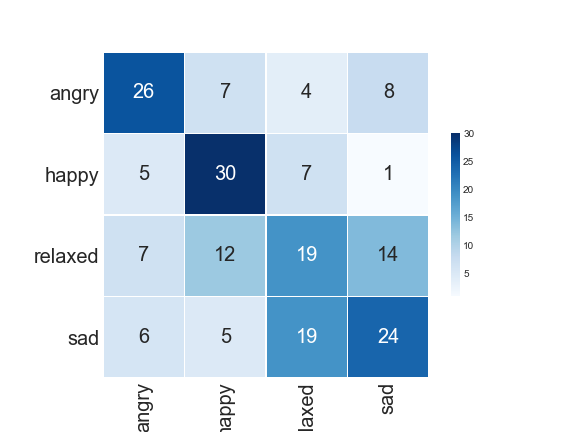
\includegraphics[width=\linewidth]{./chapters/chapter4/images/4Q/CM_ANN.png}
    \caption{ML4Q}
  \end{subfigure}
  \begin{subfigure}[b]{0.49\linewidth}
   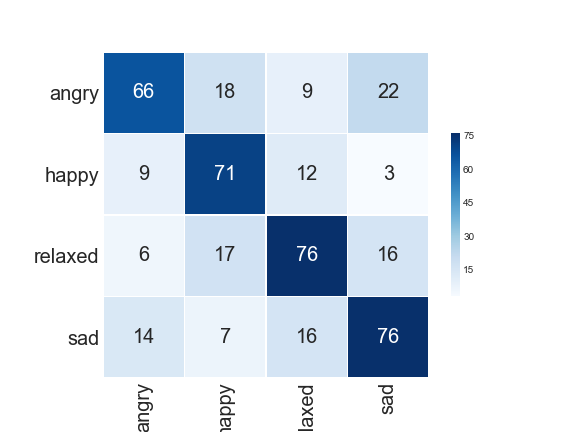
\includegraphics[width=\linewidth]{./chapters/chapter4/images/join/CM_ANN.png}
    \caption{ML + ML4Q}
  \end{subfigure}
  \caption{Artificial Neural Network - Confusion Matrix}
  \label{fig:ann}
\end{figure}

\begin{figure}[H]
  \centering
  \begin{subfigure}[b]{0.49\linewidth}
    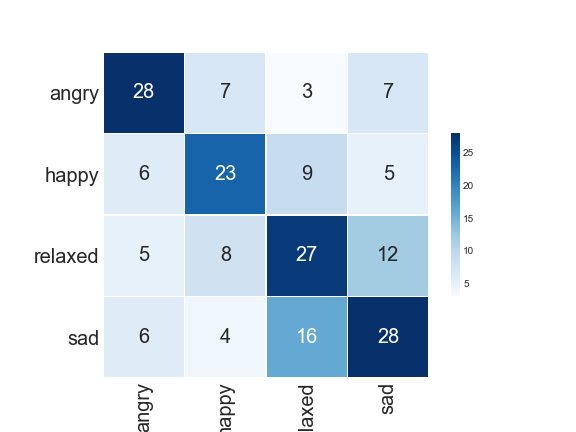
\includegraphics[width=\linewidth]{./chapters/chapter4/images/4Q/CM_LR.png}
    \caption{ML4Q}
  \end{subfigure}
  \begin{subfigure}[b]{0.49\linewidth}
   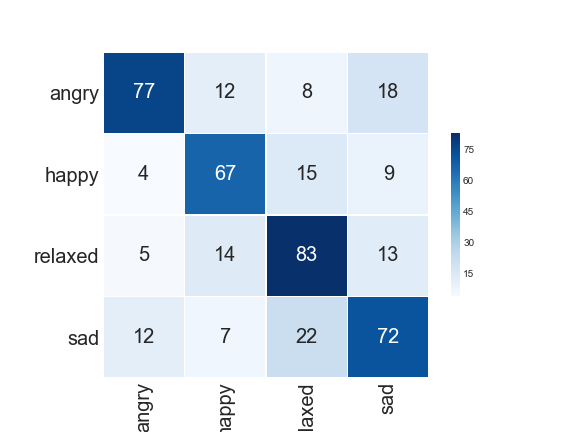
\includegraphics[width=\linewidth]{./chapters/chapter4/images/join/CM_LR.png}
    \caption{ML + ML4Q}
  \end{subfigure}
  \caption{Logistic Regression - Confusion Matrix}
  \label{fig:lr}
\end{figure}

\begin{figure}[H]
  \centering
  \begin{subfigure}[b]{0.49\linewidth}
    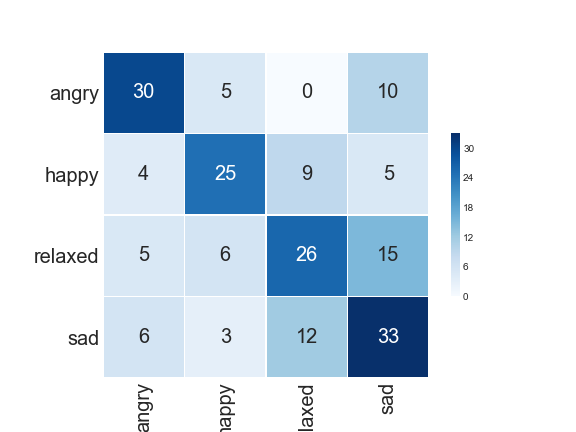
\includegraphics[width=\linewidth]{./chapters/chapter4/images/4Q/CM_SVM.png}
    \caption{ML4Q}
  \end{subfigure}
  \begin{subfigure}[b]{0.49\linewidth}
   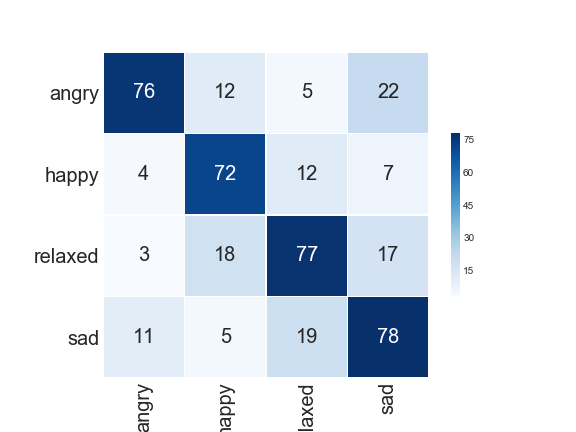
\includegraphics[width=\linewidth]{./chapters/chapter4/images/join/CM_SVM.png}
    \caption{ML + ML4Q}
  \end{subfigure}
  \caption{Support Vector Machine - Confusion Matrix}
  \label{fig:svm}
\end{figure}

\begin{figure}[H]
  \centering
  \begin{subfigure}[b]{0.49\linewidth}
    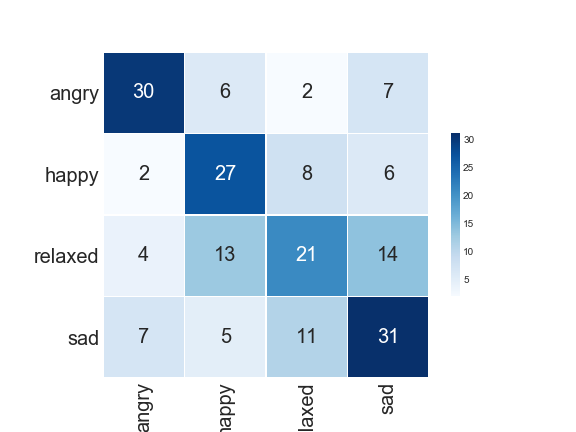
\includegraphics[width=\linewidth]{./chapters/chapter4/images/4Q/CM_XGB.png}
    \caption{ML4Q}
  \end{subfigure}
  \begin{subfigure}[b]{0.49\linewidth}
   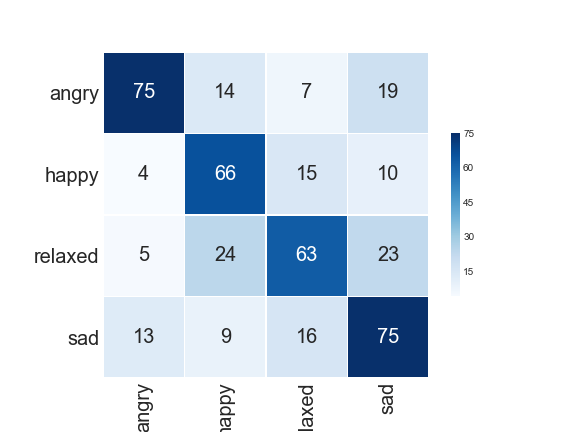
\includegraphics[width=\linewidth]{./chapters/chapter4/images/join/CM_XGB.png}
    \caption{ML + ML4Q}
  \end{subfigure}
  \caption{Xgboost - Confusion Matrix}
  \label{fig:xgb}
\end{figure}